\documentclass{beamer}
%
% Choose how your presentation looks.
%
% For more themes, color themes and font themes, see:
% http://deic.uab.es/~iblanes/beamer_gallery/index_by_theme.html
%
\mode<presentation>
{
  \usetheme{default}      % or try Darmstadt, Madrid, Warsaw, ...
  \usecolortheme{beaver} % or try albatross, beaver, crane, ...
  \usefonttheme{default}  % or try serif, structurebold, ...
  \setbeamertemplate{navigation symbols}{}
  \setbeamertemplate{caption}[numbered]
} 

\usepackage[english]{babel}
\usepackage[utf8x]{inputenc}
\usepackage{animate}
\usepackage{algorithm2e}
% COMMANDS %
\newcommand{\set}[1]{\left\{#1\right\}}
\newcommand{\abs}[1]{\left| #1\right|}
\newcommand{\eval}[1]{\mathbb{E}\left[#1\right]}
\newcommand{\var}[1]{\text{Var}\left(#1\right)}
\newcommand{\cov}[1]{\text{Cov}\left(#1\right)}
\newcommand{\prob}[1]{\mathbb{P}\left(#1\right)}
\newcommand{\borel}{\mathcal{B}([0,1])}
\newcommand{\borelR}{\mathcal{B}(\mathbb{R})}
\newcommand{\sigalg}[1]{\sigma\left(#1\right)}
\newcommand{\R}{\mathbb{R}}
\newcommand{\N}{\mathbb{N}}
\newcommand{\F}{\mathcal{F}}
\newcommand{\G}{\mathcal{G}}
\newcommand{\leb}[1]{\mu_{\text{Leb}}\left(#1\right)}
\newcommand{\limn}{\lim_{n\rightarrow\infty}}
\renewcommand{\vec}[1]{\mathbf{#1}}

\title{Control With Gradient TD Methods + The Nonlinear Case}
\subtitle{COMP 767}
\author{Matthew Smith}
\date{}

\begin{document}

\begin{frame}
  \titlepage
\end{frame}

% Uncomment these lines for an automatically generated outline.
%\begin{frame}{Outline}
%  \tableofcontents
%\end{frame}


%----------------------------------------------------------------------

\begin{frame}{Overview}

\tableofcontents
This slide is just to add slides.
\end{frame}

%----------------------------------------------------------------------
\section{Gradient TD}
\begin{frame}{The part we've covered:}

\begin{itemize}
\item This Picture:
  \begin{figure}
  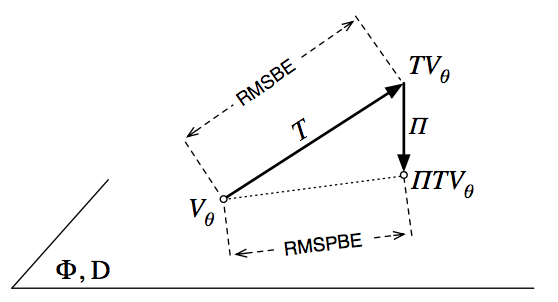
\includegraphics[width=0.8\linewidth]{classic.png}
  \end{figure}
  \item \[MSPBE = ||  (\Pi_\theta TV_\theta - V_\theta)||_D^2\]
   \[-1/2 \nabla MSPBE = - \mathbb{E}[\delta\phi]
- \gamma\mathbb{E}[\phi'\phi^\top ]w
  \]
\[w = \mathbb{E}[\phi\phi^\top]^{-1}\mathbb{E}[\delta\phi]\]
\end{itemize}

\end{frame}
\begin{frame}{The part we haven't:}

\begin{itemize}
\item This Picture:
  \begin{figure}
  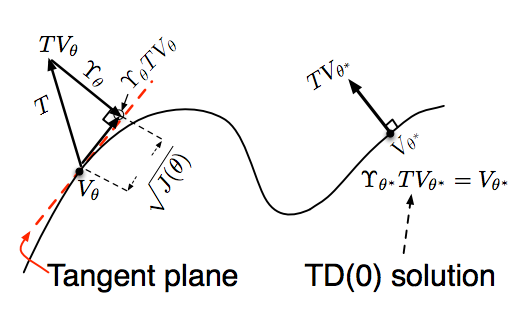
\includegraphics[width=0.7\linewidth]{woah.png}
  \end{figure}
\item MSPBE now projects onto the tangent space of the nonlinear function which we assume to be smooth enough to be locally linear.\[MSPBE = || \Pi_\theta (TV_\theta - V_\theta)||_D^2\]
 \[-1/2 \nabla MSPBE = - \mathbb{E}[\delta\phi]
- \gamma\mathbb{E}[\phi'\phi^\top]w + h(\theta, w)
  \]
\[w = \mathbb{E}[\phi\phi^\top]^{-1}\mathbb{E}[\delta\phi]\]
\end{itemize}

\end{frame}
\begin{frame}{The part we haven't:}

\begin{itemize}
\item Update rules are much the same but now there are second order terms.
\[\theta_{k+1} = \Gamma\left[\theta_k + \alpha_k\{\delta_k\phi_k - \gamma\phi_k'(\phi_k^\top w_k) - h_k\}\right]\]
\[h_k = \delta_k - (\phi_k^\top w_k) \delta^2V_\theta(s_k)w_k\]
\item note that now $\phi_k = \nabla V_\theta(s_k)$
\item Also, Lee and Anderson, 2014 do this + control with small neural nets
\end{itemize}
\end{frame}

\begin{frame}{Quick Results}
  \begin{figure}
    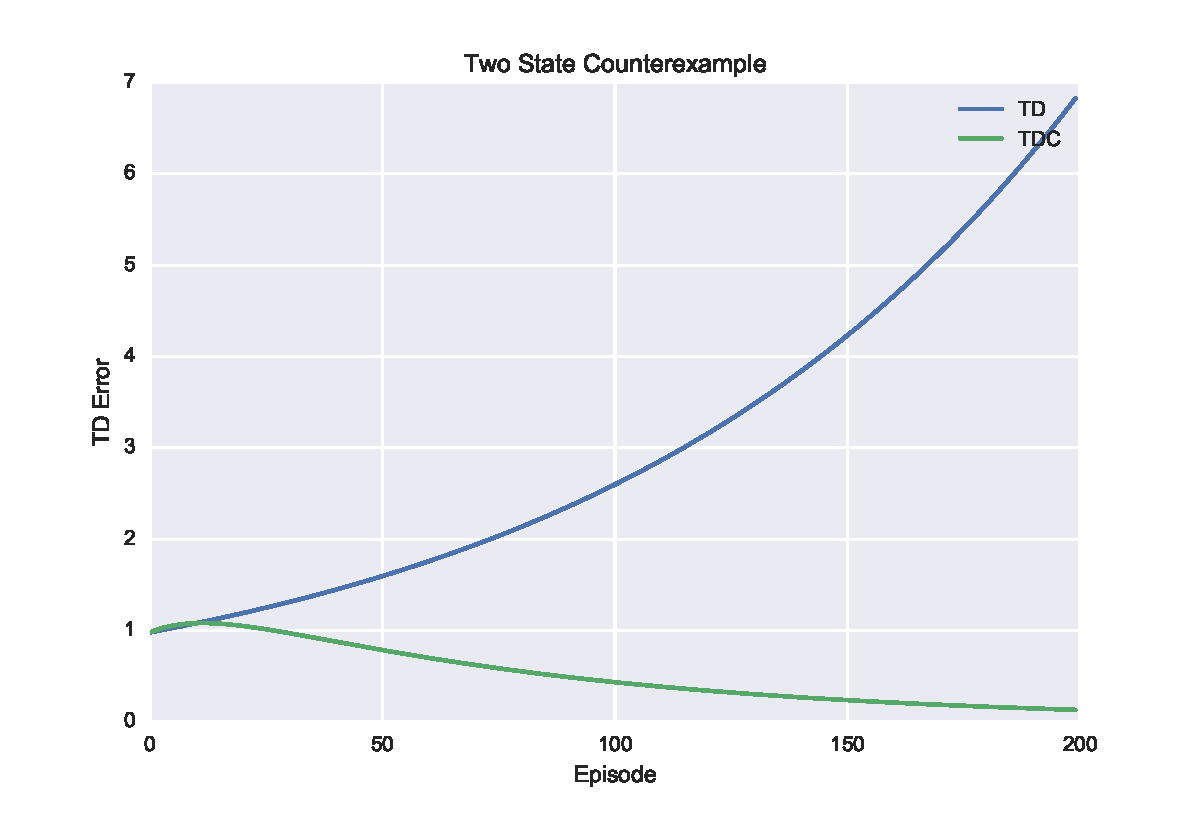
\includegraphics[width=0.7\linewidth]{2State.pdf}
  \end{figure}
\end{frame}
\begin{frame}{Quick Results}
  \begin{figure}
    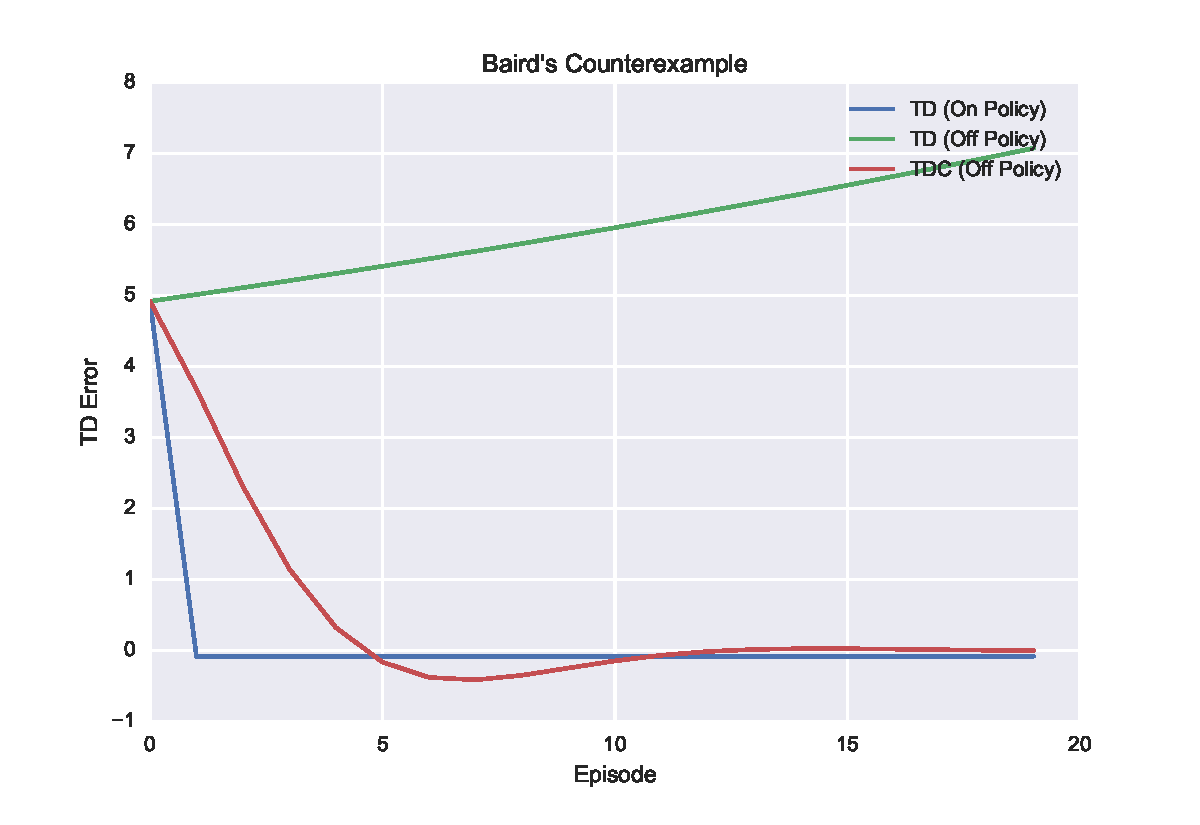
\includegraphics[width=0.7\linewidth]{Baird2.pdf}
  \end{figure}
\end{frame}
\begin{frame}{Quick Results}
  \begin{figure}
    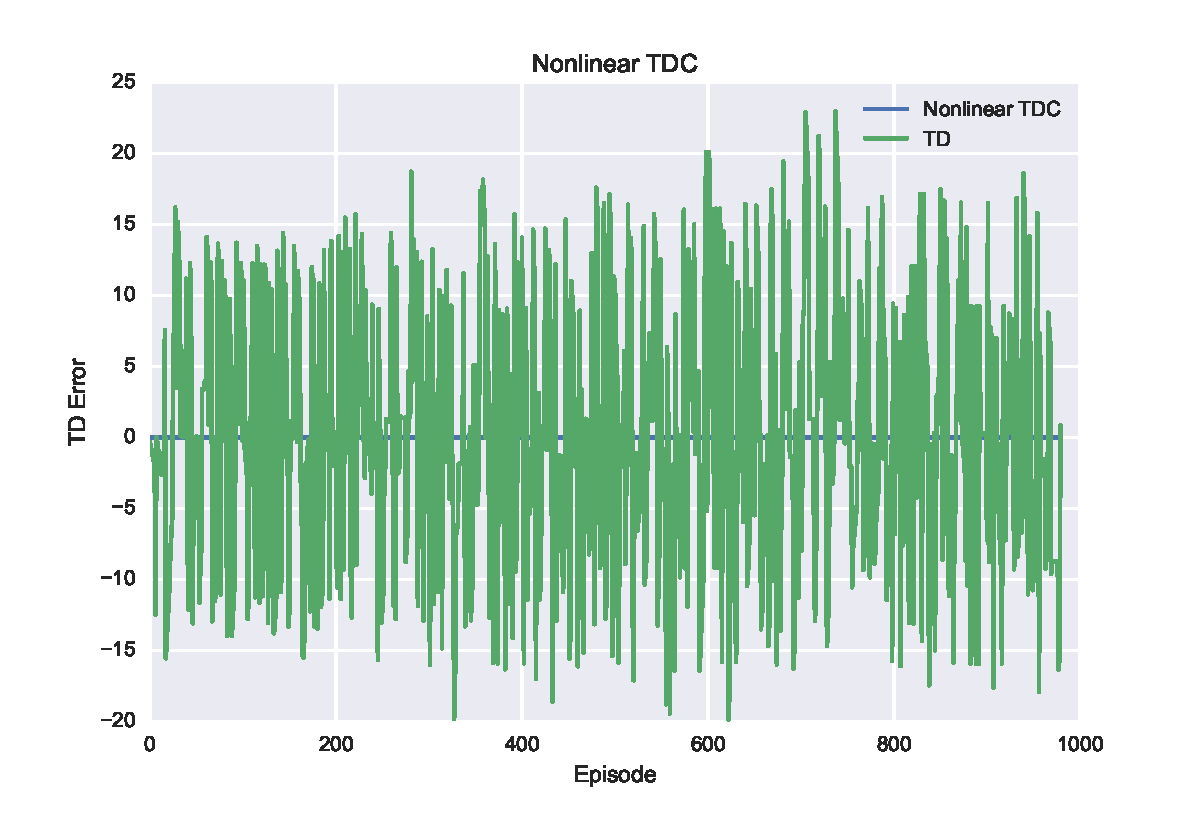
\includegraphics[width=0.7\linewidth]{NonLinTDC.pdf}
  \end{figure}
\end{frame}


\section{Control With Gradient TD Methods}
\begin{frame}{Control With Gradient TD Methods}
 \begin{algorithm}[H]
    $\theta \sim$ random\\
    $s \sim$ inital state
    \While{not terminal}{
        Choose $a$ from $\epsilon$-Greedy on $Q_\theta(s,a)$\\
        Observe $(s',r)$\\
        Choose $a' = max_i(Q_\theta(s',i))$\\
        update $Q_\theta$ according to TDC($\theta$,s,a,r,$s',a'$)\\
        $s = s' $

    }
 \caption{Greedy-QC}
\end{algorithm}
\end{frame}
\begin{frame}{Simply Plug TDC or GTD2 into SARSA or Q-learning!}
This is in the original feature space!
  \begin{figure}
    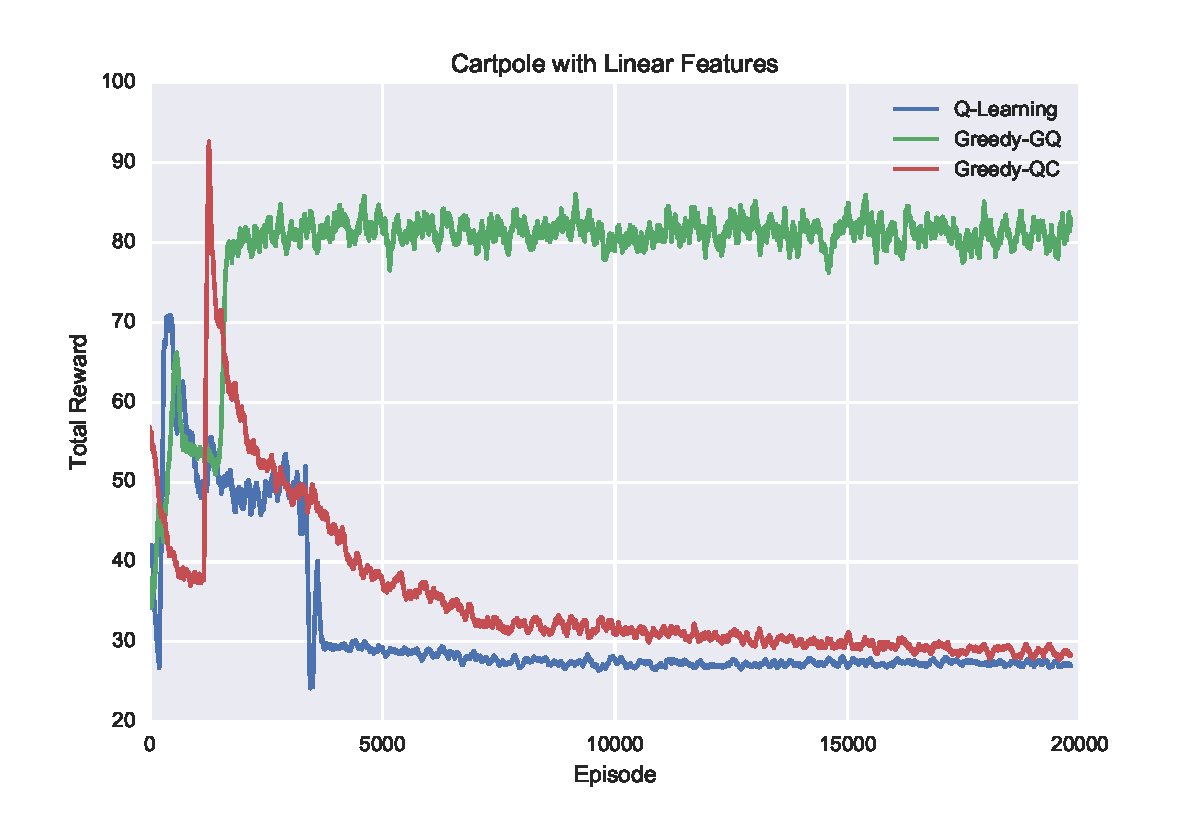
\includegraphics[width=0.7\linewidth]{LinearCartPole-GQ.pdf}
  \end{figure}
\end{frame}
\begin{frame}{Simply Plug TDC or GTD2 into SARSA or Q-learning!}
This is in the original feature space!
  \begin{figure}
    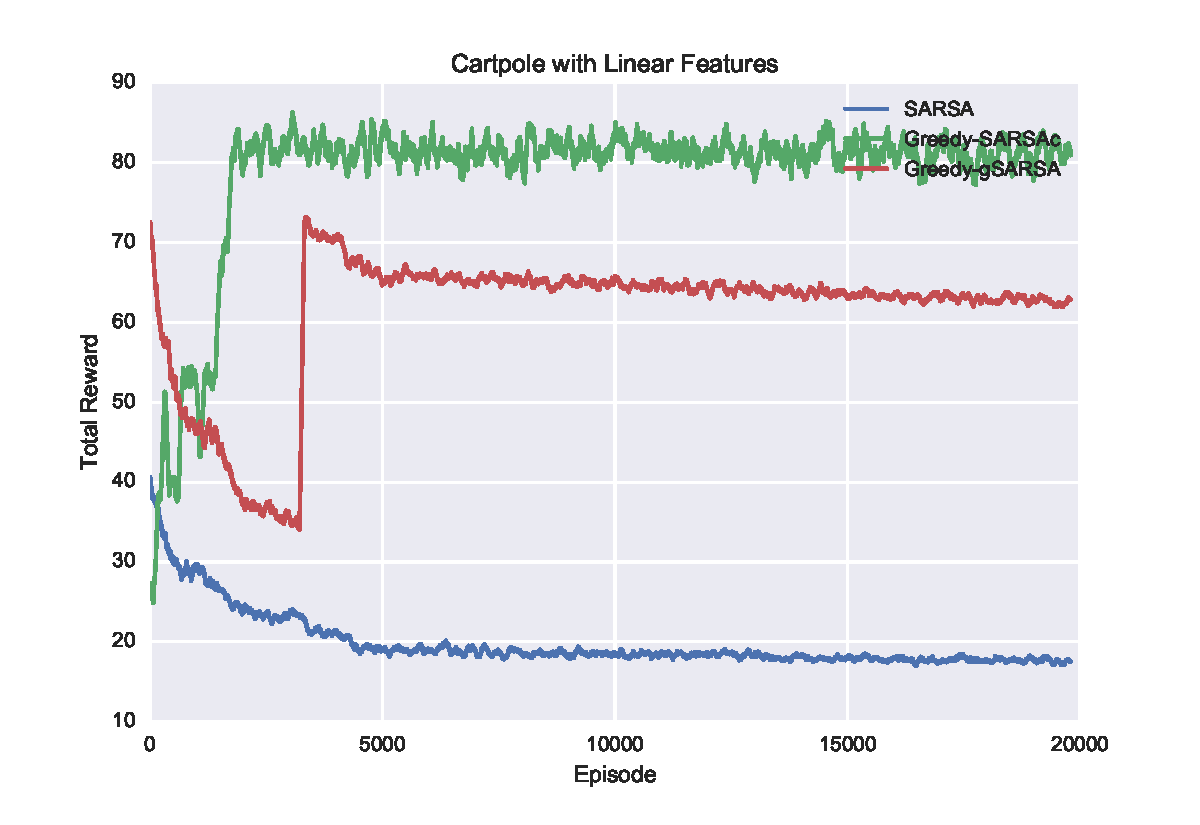
\includegraphics[width=0.7\linewidth]{LinearCartPole-GSarsa.pdf}
  \end{figure}
\end{frame}


\end{document}
%----------------------------------------------------------------------

\end{document}

